\documentclass[12pt]{report}
\usepackage{amsthm}
\usepackage{amssymb}
\usepackage{amsmath}
\usepackage[parfill]{parskip}  				% Newlines create actual paragraphs
\usepackage{algorithm} 						% For pseudocode
\usepackage{algpseudocode}  					% For pseudocode
\usepackage{hyperref}						% Adds hyperlinks
\usepackage{bm}								% Bold math
\usepackage{tikz}							% Graph drawing
\usepackage{subcaption}						% Subfigures

% Add spacing between theorems, which is zeroed by parskip
\makeatletter
\def\thm@space@setup{%
  \thm@preskip=\parskip \thm@postskip=0pt
}
\makeatother

% algpseudocode modifications
\renewcommand{\algorithmicrequire}{\textbf{Input:}}
\renewcommand{\algorithmicensure}{\textbf{Output:}}
\algnewcommand{\Continue}{\State \textbf{continue}}

% Theorem keyword definitions
\newtheorem{theorem}{Theorem}[chapter]
\newtheorem{definition}[theorem]{Definition}
\newtheorem{proposition}[theorem]{Proposition}
\newtheorem{lemma}[theorem]{Lemma}
\newtheorem{corollary}[theorem]{Corollary}

\title{
{Pathfinding algorithms in graphs and applications}\\
{\large Universitat de Barcelona}
}
\author{Daniel Monzonís Laparra}

\begin{document}
\maketitle

\chapter*{Abstract}
Abstract goes here.

\tableofcontents

\chapter{Introduction}
Many problems in the fields of science, mathematics and engineering can be generalised to the problem of finding a path in a graph. Examples of such problems include routing of telephone or Internet traffic, layout of printed circuit boards, automated theorem proving, GPS routing, decision making in artificial intelligence and robotics. In this article, we will provide a mathematical and applied approach to this problem.

For most of the examples in the article we will be using a grid graph, represented by a tiled 2D map, in which each tile (or node) is connected to its adjacent tiles. In the map, each tile can have a different weight, or be a wall, which is impassable. This notion of weighted nodes and walls can be translated to the structure of a weighted directed graph by thinking of the weights of the tiles as the weights of the edges that connect adjacent tiles to it. Walls can be thought of as nodes that are not connected (or just non-existent) to any other node, and therefore not reachable from other nodes. A pathfinding simulator was built for this article to help illustrate these examples.

\chapter{The $A^*$ algorithm}
The $A^*$ algorithm is a very popular algorithm used in many applications to find the optimal path between two points. The algorithm works on graphs, a structure well studied in graph theory, so first we will refresh some definitions.

\begin{definition}
A \textbf{directed graph} $G$ is a pair of sets $(V, E)$, where $V$ is the set of vertices or nodes, and $E$ the set of edges, formed by pairs of vertices.
\end{definition}

\begin{definition}
A \textbf{weighted directed graph} is a graph in which $\forall e \in E \ \exists w(e) \in \mathbb{R}$. We call $w(e)$ the \textbf{weight} or \textbf{cost} of the edge $e$.

If $e = (u, v)$ for some $u, v \in V$, then we equivalently call $d(u, v) = w(e)$ the \textbf{distance} from $u$ to $v$.
\end{definition}

From now on, when we talk about a graph, we will implicitly refer to a finite weighted directed graph, since it's the most general type of graph we will work with. An unweighted graph can be thought of as a weighted graph where all weights are equal to one, and an undirected graph as a directed graph where $\forall (u, v) \in E,\  \exists (v, u) \in E$. Also, the graphs we will work with are finite, meaning that $|V| < \infty$ and $|E| < \infty$.

\begin{definition}[Path]
Given a graph $G$, and $u, v \in V$, a \textbf{path} $P$ between $u$ and $v$ is an ordered list of a certain amount of edges, $N$, in the form

\[ P = \{(u,v_1), (v_1, v_2), \dots, (v_{N-2}, v_{N-1}), (v_{N-1}, v)\} \]

\end{definition}

Note that paths are not unique. There may exist multiple paths between two nodes.

\begin{definition}
We say that two nodes $u, v \in V$ are connected $\Longleftrightarrow$ There exists a path $P$ between $u$ and $v$.
\end{definition}

\begin{definition}
Given a path $P$ between two nodes $u, v \in V$, given a node $n$ which is in the path, we say that $n'$ is the \textbf{successor} of $n$ if $(n, n') \in P$, that is, if we followed the path $P$, the next node we would visit when we have reached $n$ would be $n'$.
\end{definition}

\begin{definition}
If $u \in V$, we define the \textbf{connected component} of $u$ as
\[ C_u = \{ v \in V\ |\ u \ \text{and} \ v \ \text{are connected}\  \} \]
\end{definition}

\begin{definition}[Distance of a path]
Given a path $P$ in a weighted directed graph $G$, we define the \textbf{weight} or \textbf{distance} of the path, $dist(P)$, as

\[ d(P) = \sum_{e \in P} w(e) \]

If $P$ is a path between $u$ and $v$, we can equivalently write

\[ d_P(u, v) = d(P) \]

If the context is clear, we will just write $d(u, v)$. For convenience, if $u$ and $v$ are not connected, we define the distance between them as $d(u, v) = \infty$.
\end{definition}

Note that, in general, $d(u, v) \neq d(v, u)$, since graphs can be directed and not all paths may be reversible.

\begin{definition}[Optimal path]
\label{def:optimal}
Given a set of all the existing paths between two nodes $u$ and $v$, $\chi_{(u, v)}$, we will say that a path $P \in \chi_{(u,v)}$ is \textbf{optimal} if and only if $d(P) \le d(P') \ \forall P' \in \chi_{(u, v)}$.
\end{definition}

We will also say that $P$ is the \textbf{shortest distance path} if it is optimal, and we will write the distance that fulfils the condition in definition \ref{def:optimal} as $\delta(u,v)$. Clearly, in a finite graph, an optimal path between any two nodes always exists, since in this case $\chi_{(u, v)}$ is finite.

Instead of presenting the $A^*$ algorithm without any background, we will first briefly discuss some other widely known algorithms that can be used to find paths between nodes in graphs, and build up to the main algorithm by trying to gradually improve the performance.

\section{BFS}
Breadth-First Search, or BFS for short, attempts to find a path by methodically examining all the neighbours of each node it examines.

The algorithm uses a queue to keep track of the next nodes to examine, adding all unvisited neighbours of a node when it is examined, until the queue is empty. Explored nodes are kept in a set, so that we don't explore the same node twice. The set of nodes that haven't been explored yet is often called the \emph{open set}, and the set of visited nodes the \emph{closed set}.

The pseudocode for the algorithm is presented in algorithm \ref{alg:bfs}. The algorithm returns a map called \emph{previous}, which maps every node to the node we came from in the path that the algorithm computes. The procedure that we will use to reconstruct the path from this map for all algorithms is presented in algorithm \ref{alg:reconstruct}.

\begin{algorithm}
\caption{Breadth-First Search}
\label{alg:bfs}
\begin{algorithmic}[1]
\Procedure{BFS}{$G, \alpha, \beta$}
\Require Graph $G = (V, E)$, directed or undirected; source node $\alpha \in V$; goal node $\beta \in V$
\Ensure Given $u \in G$, previous[$u$] gives us the node come from to reach $u$ in the path computed
\State Q $\gets Queue()$
\State S $\gets Set()$ \Comment{Keeps track of explored nodes}
\State previous $\gets Map()$
\For {u $\in G$}
	\State previous[u] $\gets$ null
\EndFor
\State Q.enqueue($\alpha$)
\State S.add($\alpha$)
\While {not Q.empty()}
	\State u $\gets$ Q.front()
	\State Q.dequeue()
	\For {v $\in$ u.neighbours()}
		\If {v $\not\in$ S}
			\State Q.enqueue(v)
			\State S.add(v)
			\State previous[v] $\gets$ u
		\EndIf
	\EndFor
\EndWhile
\State \Return ReconstructPath(previous, $\alpha$, $\beta$)
\EndProcedure
\end{algorithmic}
\end{algorithm}

\begin{algorithm}
\caption{Reconstruct path}
\label{alg:reconstruct}
\begin{algorithmic}[1]
\Procedure{ReconstructPath}{previous, $\alpha$, $\beta$}
\Require The map $previous$ returned by the pathfinding algorithm; source node $\alpha \in V$; goal node $\beta \in V$
\Ensure An ordered list $P$ with the nodes from the path from $\alpha$ to $\beta$
\State $P \gets$ []  \Comment{Empty array for the path}
\State u $\gets \beta$
\While {u $\neq \alpha$}
	\State $P$.push(u)
	\State u $\gets$ previous[$\beta$]
\EndWhile
\State $P$.push($\alpha$)
\State \Return $P$.reversed()
\EndProcedure
\end{algorithmic}
\end{algorithm}

We see that with this version of BFS, all nodes in the connected component of the starting node are explored. We can improve performance if we perform an early exit, since we don't need to keep exploring once we find the end node, as shown in algorithm \ref{alg:bfs_early_exit}.

\begin{algorithm}
\caption{Breadth-First Search with early exit}
\label{alg:bfs_early_exit}
\begin{algorithmic}[1]
\Procedure{BFS}{$G, \alpha, \beta$}
\Require Graph $G = (V, E)$, directed or undirected; source node $\alpha \in V$; goal node $\beta \in V$
\Ensure Given $u \in G$, previous[$u$] gives us the node come from to reach $u$ in the path computed, if it has been explored
\State Q $\gets Queue()$
\State S $\gets Set()$
\State previous $\gets Map()$
\For {u $\in G$}
	\State previous[u] $\gets$ null
\EndFor
\State Q.enqueue($\alpha$)
\State S.add($\alpha$)
\While {not Q.empty()}
	\State u $\gets$ Q.front()
	\State Q.dequeue()
	\For {v $\in$ u.neighbours()}
		\If {v $\not\in$ S}
			\If {v $= \beta$} \Comment{Early exit condition}
				\State \Return ReconstructPath(previous,$\alpha$,$\beta$)
			\EndIf
			\State Q.enqueue(v)
			\State S.add(v)
			\State previous[v] $\gets$ u
		\EndIf
	\EndFor
\EndWhile
\EndProcedure
\end{algorithmic}
\end{algorithm}

Note that, even though BFS will always find a path between two nodes if they are connected, the path produced is not optimal when we consider weights. The path found will be the shortest in terms of the number of steps, but when taking into account the weights of the edges, this algorithm will not give us the shortest distance path, as we can see in figure \ref{fig:bfs-fail}.

%TODO Put example images
\begin{figure}
\centering
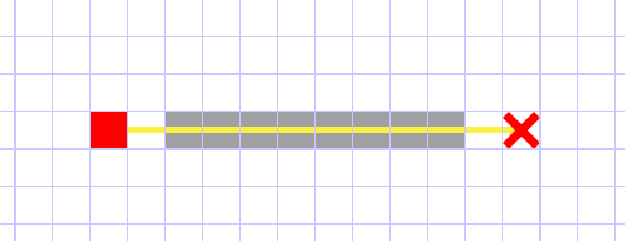
\includegraphics[width=1\linewidth]{bfs-fail}
\caption{An example on how BFS fails to find an optimal path when we use a weighted graph. In this example, moving to a white tile has cost 1, while moving to a gray tile has cost 10, so clearly, going in a straight line is not the optimal path.}
\label{fig:bfs-fail}
\end{figure}


Also, the algorithm doesn't seem very efficient, since we can potentially explore lots of nodes on a very dense graph.

We will first address the optimality problem in the next algorithm, and then we will focus on efficiency.

\section{Dijkstra}
The Dijkstra algorithm is also a well known graph theory algorithm, used to find the optimal path between two nodes in a graph with positive weights. Now, instead of a simple queue, we use a priority queue. We keep exploring all unvisited neighbours of a node, but now we insert them in the priority queue using the distance of the edge.

Normally, the algorithm only gets a starting node, and computes the optimal paths to all reachable nodes from the origin, but since we're only concerned about finding the path from one specific node to another, we will use the early exit condition to end the execution as soon as we explore the goal node. We will later see that this still gives us the optimal path.

\begin{algorithm}
\caption{Dijkstra's algorithm}
\label{alg:dijkstra}
\begin{algorithmic}[1]
\Procedure{Dijkstra}{$G$, $\alpha$, $\beta$}
\Require Graph $G = (V, E)$, directed or undirected; source node $\alpha \in V$; goal node $\beta \in V$
\Ensure Given $u \in G$, previous[$u$] gives us the node come from to reach $u$ in the path computed, and d[$u$] gives us the distance to that node, if it has been explored
\State Q $\gets PriorityQueue()$
\State S $\gets Set()$
\State d $\gets Map()$ \Comment{Keeps track of the shortest distance to each node}
\State previous $\gets Map()$
\For {u $\in G$}
	\State d[u] $\gets \infty$
	\State previous[u] $\gets$ null
\EndFor
\State Q.insert((0, $\alpha$))
\State d[$\alpha$] $\gets 0$
\While {not Q.empty()}
	\State u $\gets$ Q.removeMin()
	\State S.add(u)
	\If {u $= \beta$} \Comment{Early exit condition}
		\State \Return ReconstructPath(previous,$\alpha$,$\beta$)
	\EndIf
	\For {v $\in$ u.neighbours()}
		\If {v $\in S$}
			\Continue \Comment{Already explored node}
		\EndIf
		\State alt $\gets$ d[u] $+ w((u, v))$
		\If {alt $<$ d[v]}
			\State d[v] $\gets$ alt
			\State Q.insert((v, alt))
			\State previous[v] $\gets$ u
		\EndIf
	\EndFor
\EndWhile
\EndProcedure
\end{algorithmic}
\end{algorithm}

We will now prove the correctness of the algorithm without the early exit condition, that is, given a node $u \in V$, the algorithm always finds the optimal path between $u$ and all other nodes $v \in V$ such that $u$ and $v$ are connected. We will do so by induction on the visited set used in algorithm \ref{alg:dijkstra}, which we will call $S$. We will also write the distance computed by Dijkstra's algorithm between two nodes $u, v$ as $d_D(u, v)$.

\begin{lemma}
\label{lemma:dijkstra}
At any given step of the algorithm, $\forall s \in S,\ d_D(u, s) = \delta(u, s)$
\end{lemma}
\begin{proof}
If $|S| = 0$, the statement is trivially true.

If $|S| = 1$, it must be $S = \{u\}$, since $S$ only grows in size, but $d_D(u, u) = 0 = \delta(u, u)$.

Now let's assume we are in an arbitrary step, and let $s$ be the current node being explored, not yet added to $S$. Let $S' = S \cup \{s\}$. By inductive hypothesis, we know that $\forall t \in S,\ d_D(u, t) = \delta(u, t)$. Now we only need to show that $d_D(u, s) = \delta(u, s)$.

Suppose that there exists a path $Q$ from $u$ to $s$ such that
\[d(Q) < d_D(u, s)\]
We know that the path $Q$ starts in $S$ (since $u \in S$), but at some point has to leave $S$ (since $s \not\in S$). Let $e = (x, y) \in Q \subset E$ be the first edge that leaves $S$, that is, $x \in S$ but $y \not\in S$. Let $Q_x \subset Q$ be the edges of $Q$ up until and without including the edge $e$. Clearly,
\[d(Q_x) + d(x, y) \le d(Q)\]

By the induction hypothesis, $d_D(u, x) = \delta(u, x) \le d(Q_x)$. Therefore,
\[ d_D(u, x) + d(x, y) \le d(Q) \]

Clearly, $\delta(u, y) \le d_D(u, x) + d(x, y)$.

Since $y \not\in S$, and since Dijkstra uses a priority queue to select the next reachable node with minimum distance, we know that $d_D(u, s) \le d_D(u, y)$.

Combining the inequalities, we get that
\[ d_D(u, s) \le d_D(u, y) \le d_D(u, x) + d(x, y) \le d(Q) < d_D(u, s) \]
which is a contradiction.

Therefore, $d_D(u, s) = \delta(u, s)$.
\end{proof}

\begin{theorem}[Correctness of Dijkstra's algorithm]
\label{thm:dijkstra}
Let $G = (V, E)$ be a weighted directed graph. Let $u \in V$. Then, after running Dijkstra's algorithm with start node $u$, the following is true
\[ \forall v \in C_u,\  d_D(u, v) = \delta(u, v) \]
\end{theorem}
\begin{proof}
We know that, at the end of Dijkstra's algorithm, we'll have explored all the nodes connected to $u$. That is, $S = C_u$. For each $v \in C_u$, apply \ref{lemma:dijkstra} to get the wanted result.
\end{proof}

Like with BFS, we can modify the algorithm to use early exit to improve performance.
\begin{lemma}
Using Dijkstra's algorithm with early exit with start node $u$ and end node $v$ ensures that $d_D(u, v) = \delta(u, v)$.alt
\end{lemma}
\begin{proof}
With early exit, when we explore node $v$ we will end the execution of the algorithm. Using \ref{lemma:dijkstra}, we know that $d_D(u, v) = \delta(u, v)$, so we already have the optimal path between the two nodes.
\end{proof}

% TODO: Talk about what happens when there are negative weights. Name Bellman-Ford algorithm.
Note that Dijkstra's algorithm only works for graphs with positive weights. For graphs with negative weights, there are other less efficient algorithms which also find optimal paths, like the Bellman-Ford algorithm.

\section{Greedy Best-First search}
\label{section:greedy}
As we have seen in the last section, we now have an algorithm that can find the optimal path between any two nodes in a graph with positive weights. We will now start to worry about improving the performance of the algorithms.

Let's forget about optimality for a while, and modify our pathfinding algorithm to use only an heuristic. An heuristic is a function
\begin{align*}
	h \colon V &\to \mathbb{R}\\
	u &\mapsto h(u)
\end{align*}
which gives an estimate of the true distance from a node to the goal node, which we compute without having to expand extra nodes, and varies with each type of problem we have.

We will talk more about heuristics later, but for now, let's consider what happens when we use heuristics instead of the actual distance of the paths between nodes, like we did in Dijkstra's algorithm, for the priority queue ordering. 

In Dijkstra, we used the actual distances of the paths between nodes for the priority queue ordering. Now, we will use the heuristic, so that the node closest to the goal will be the first to be explored.

\begin{algorithm}
\caption{Greedy Best-First search}
\label{alg:greedy}
\begin{algorithmic}[1]
\Procedure{GreedyBestFirstSearch}{$G$, $\alpha$, $\beta$}
\Require Graph $G = (V, E)$, directed or undirected; source node $\alpha \in V$; goal node $\beta \in V$
\Ensure Given $u \in G$, previous[$u$] gives us the node come from to reach $u$ in the path computed, if it has been explored
\State Q $\gets PriorityQueue()$
\State S $\gets Set()$
\State previous $\gets Map()$
\For {u $\in G$}
	\State previous[u] $\gets$ null
\EndFor
\State Q.insert((0, $\alpha$))
\While {not Q.empty()}
	\State u $\gets$ queue.removeMin()
	\State S.add(u)
	\If {u $= \beta$} \Comment{Early exit condition}
		\State \Return ReconstructPath(previous,$\alpha$,$\beta$)
	\EndIf
	\For {v $\in$ u.neighbours()}
		\If {v $\in S$}
			\Continue
		\EndIf
		\State Q.insert((v, $h(v)$))
		\State previous[v] $\gets$ u
	\EndFor
\EndWhile
\EndProcedure
\end{algorithmic}
\end{algorithm}

%TODO Define tilemap as 2d discrete map
%TODO Define manhattan distance
%\begin{definition}
%The \textbf{Manhattan distance} between two points %TODO FINISH
%\end{definition}

%TODO Talk about the problems with the greedy search

\section{$A^*$}
As we have seen, Dijkstra always gives us optimal paths, but it wastes a lot of time exploring a lot of nodes that are not in a promising direction. On the other hand, Greedy Best-First Search explores nodes in a promising direction, but does not produce optimal paths reliably.

The $A^*$ algorithm is a combination of both algorithms. It takes into account both the actual distance from the source to a node, and the estimated distance from the node to the goal. Unlike Dijkstra's algorithm, which works for positive weights, $A^*$ only works with strictly positive weights.

Given two connected nodes $\alpha, \beta \in V$, consider the optimal path between $\alpha$ and $\beta$, $P$. For any node $u$ that is part of $P$, we define a function $\hat{f}(u) = \hat{g}(u) + \hat{h}(u)$, where $\hat{g}(u) = \delta(\alpha, u)$ and $\hat{h}(u) = \delta(u, \beta)$. Note that for any other node $v$ in the optimal path $P$, $\hat{f}(u) = \hat{f}(v)$.

Now suppose we have functions $g(u)$ and $h(u)$ which give us estimates for $\hat{g}(u)$ and $\hat{h}(u)$ respectively.

\begin{definition}
Given a source and goal nodes in a graph $G = (V, E)$, we define the \textbf{score} as the function
\begin{align*}
	f \colon V &\to \mathbb{R}\\
	u &\mapsto f(u) = g(u) + h(u)
\end{align*}
where $g(u)$ is an estimate of the optimal distance from the source to the node $u$, and $h(u)$ is an estimate of the optimal distance from the node $u$ to the goal.
We will call $g$ the \textbf{g-score}, and $h$ the \textbf{h-score}.
\end{definition}

In $A^*$, a good choice for the g-score is using, for each node $u$, the cost of the path from the source to $u$ found so far by the algorithm, which would be equivalent to the distance map we kept updating in Dijkstra's algorithm. Note that this implies $g(u) \geq \hat{g}(u) \ \forall u \in V$. For the h-score, we will use some heuristic.

When a node is explored, its g-score, and thus its score will be updated. The pseudocode for the algorithm is shown in algorithm \ref{alg:astar}. As we can see, it's very similar to Dijkstra's, except that we now use the score for the priority queue ordering, instead of just the distance to that node.

\begin{algorithm}
\caption{$A^*$ algorithm}
\label{alg:astar}
\begin{algorithmic}[1]
\Procedure{AStar}{$G$, $\alpha$, $\beta$}
\Require Graph $G = (V, E)$, directed or undirected; source node $\alpha \in V$; goal node $\beta \in V$
\Ensure Given $u \in G$, previous[$u$] gives us the node come from to reach $u$ in the path computed, and g[$u$] is the current g-score of the node
\State Q $\gets PriorityQueue()$
\State S $\gets Set()$
\State g $\gets Map()$
\State previous $\gets Map()$
\For {u $\in G$}
	\State g[u] $\gets \infty$
	\State previous[u] $\gets$ null
\EndFor
\State Q.insert((0, $\alpha$))
\State g[$\alpha$] $\gets 0$
\While {not Q.empty()}
	\State u $\gets$ Q.removeMin()
	\State S.add(u)
	\If {u $= \beta$} \Comment{Early exit condition}
		\State \Return ReconstructPath(previous,$\alpha$,$\beta$)
	\EndIf
	\For {v $\in$ u.neighbours()}
		\If {v $\in S$}
			\Continue \Comment{Already explored node}
		\EndIf
		\State alt $\gets$ g[u] $+ w((u, v))$
		\If {alt $<$ g[v]}
			\State g[v] $\gets$ alt \Comment{Update the g-score}
			\State $f = g[v] + h(v)$
			\State Q.insert((v, f))
			\State previous[v] $\gets$ u
		\EndIf
	\EndFor
\EndWhile
\EndProcedure
\end{algorithmic}
\end{algorithm}

%TODO is this paragraph necessary...?
This new algorithm is faster than Dijkstra, but it only finds optimal paths within a certain condition, which is what we will prove next.

\begin{definition}
A heuristic $h$ is said to be \textbf{admissible} if and only if, $\forall u \in V$, $h(u)$ never overestimates the real cost of moving from $u$ to the goal, that is, given a goal node $v \in V$, then $\forall u \in V \ h(u) \le \hat{h}(u) = \delta(u, v)$.
\end{definition}

We will prove that, with the score function we have constructed, $A^*$ finds optimal paths as long as the heuristic is admissible. Consider a graph $G = (V, E)$, a source node $\alpha$ and a goal node $\beta$, such that $\alpha$ and $\beta$ are connected. Consider the closed set $S$, which corresponds to the set of visited nodes in the algorithm, and the open set $O$, which are the nodes that haven't been explored yet.

\begin{lemma}
\label{lemma:astar1}
 For any node $u \not \in S$ and for any optimal path $P$ from $\alpha$ to $u$, $\exists v \in O$ which is part of $P$ such that $g(v) = \hat{g}(v)$.
\end{lemma}
\begin{proof}
Consider an optimal path from $\alpha$ to $u$,
\[P = \{ (u_0 = \alpha, u_1), (u_1, u_2), \dots, (u_{n-1}, u_n = u) \}\]

If $v = \alpha$, which implies that $\alpha \in O$, so the algorithm hasn't completed the first iteration yet, then the lemma is trivially true since $g(\alpha) = \hat{g}(\alpha) = 0$.

Now suppose $\alpha \in S$. Let
\[ \Delta = \{ n \in S \  | \  n \text{ is part of } P,\  g(n) = \hat{g}(n) \} \]
$\Delta$ is clearly not empty since $\alpha \in \Delta$.

Let $n^* \in \Delta$ be the node that satisfies $d_P(\alpha, n^*) \leq d_P(\alpha, n) \  \forall n \in \Delta$. Since $w(e) > 0\  \forall e \in E$, $n^*$ is unique. Also, $n^* \neq u$ since $u \not \in S$. Let $v$ be the successor of $n^*$ in $P$. Note that it's possible that $v = u$.

Now, $g(v) \leq g(n^*) + w((n^*, v))$ by the definition of $g$, and since $n^* \in \Delta$, $g(n^*) = \hat{g}(n^*)$. Also, $\hat{g}(v) = \hat{g}(n^*) + w((n^*, v))$, because $P$ is an optimal path. Therefore, $g(v) \leq \hat{g}(v)$. But it is always true that $g(v) \geq \hat{g}(v)$. Therefore, $g(v) = \hat{g}(v)$, and by the definition of $\Delta$, $v \not \in \Delta$ implies $v \in O$.
\end{proof}

\begin{lemma}
\label{lemma:astar2}
Suppose the heuristic used by $A^*$ is admissible, and suppose $A^*$ has not terminated. Then, for any optimal path $P$ from $\alpha$ to $\beta$, $\exists v$ in $P$ with $f(v) \leq \hat{f}(\alpha)$.
\end{lemma}
\begin{proof}
By lemma \ref{lemma:astar1}, $\exists v$ in $P$ with $g(v) = \hat{g}(v)$. Therefore, by the definition of the score function and the hypothesis,
\begin{align*}
f(v) &= g(v) + h(v)\\
&= \hat{g}(v) + h(v)\\
&\leq \hat{g}(v) + \hat{h}(v) = \hat{f}(v)
\end{align*}
Since $P$ is an optimal path, $\hat{f}(v) = \hat{f}(\alpha) \  \forall v$ in the path $P$, which proves the lemma.
\end{proof}

\begin{theorem}[Correctness of $A^*$]
\label{thm:astar}
If the heuristic is admissible, then $A^*$ always finds an optimal path between two connected nodes.
\end{theorem}
\begin{proof}
There are only three possible cases in which $A^*$ doesn't find an optimal path: the algorithm terminates at a node which is not the goal, terminates at the goal node but the path found isn't optimal, or fails to terminate at all. Let's consider the three cases separately.

Consider the case where the algorithm terminates at a node which is not the goal. Since we are using the early exit condition, which makes the algorithm terminate whenever it puts the goal node in the closed set, the only possible way that the algorithm terminates without having found the goal node is if the goal node was never in the open set to start with, or equivalently, the goal node is not connected to the start node, which contradicts our hypothesis.

Consider the case where the algorithm terminates at the goal node, but doesn't find an optimal path. Note that since the heuristic is admissible
\[ 0 \leq h(\beta) \leq \hat{h}(\beta) = 0 \  \Rightarrow \  h(\beta) = 0 \]
In this case, by the time the algorithm terminates, we have $f(\beta) = g(\beta) > \hat{f}(\alpha)$ because the path found is not optimal. But by lemma \ref{lemma:astar2}, just before termination, there existed a node $u \in O$ on an optimal path with $f(u) \leq \hat{f}(\alpha) < f(\beta)$, and since the algorithm uses a priority queue with the score, the node $u$ would have been selected for expansion instead of $\beta$, and the algorithm wouldn't have terminated.

Finally, consider the case where the algorithm fails to terminate. Remember that in $A^*$ we only work with graphs in which weights are strictly positive. Let 
\[ \epsilon = \min_{e \in E} w(e) > 0 \]
For any node $u$ further than $M = \hat{f}(\alpha) / \epsilon$ steps from $\alpha$, we have
\[ f(u) \geq g(u) \geq \hat{g}(u) > M \epsilon = \hat{f}(\alpha) \]
By lemma \ref{lemma:astar2}, we see that there is a node $v \in O$ on an optimal path such that $f(v) \leq \hat{f}(\alpha) < f(u)$, so the algorithm will always pick it first, and therefore no nodes further than $M$ steps from $\alpha$ are ever explored.

Then, the only reason why the algorithm never terminates is because it's trapped in a loop where it repeatedly explores nodes that are less than $M$ steps away from $\alpha$. Let $V_M$ be the set of nodes accessible within $M$ or less steps from $\alpha$. Consider any node $u \in V_M$. There are only a finite number of paths from $\alpha$ to $u$ that only pass through nodes in $V_M$, and therefore $u$ can only be explored a finite number of times. We call this number $m_u$. Let
\[ m = \max_{u \in V_M} m_u \]
which is the maximum number of times any node can be explored. Then, after at most $|V_M| \cdot m$ expansions, all nodes in $V_M$ will be in the closed set. But we've seen that no nodes outside $V_M$ can be explored. Therefore, $A^*$ must terminate.
\end{proof}

%TODO reference manhattan distance which will be defined in a future chapter
In figure \ref{fig:counterexample:admissible} we see a counterexample of how the converse is not true in general. Here, we are using the Manhattan distance as heuristic, which is an inadmissible heuristic if diagonal movement is allowed, since it will overestimate the true optimal distance between nodes. We can see that $A^*$ finds a path with distance $23$, which is not optimal because, in the same circumstances, Dijkstra finds a path with distance $16$.

\begin{figure}
\centering
\begin{subfigure}[b]{0.65\textwidth}
	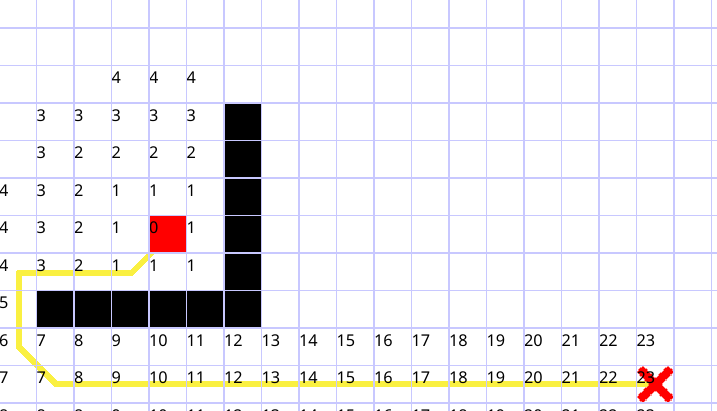
\includegraphics[width=1\linewidth]{astar-fail}
	\caption{$A^*$}
\end{subfigure}
\begin{subfigure}[b]{0.65\textwidth}
	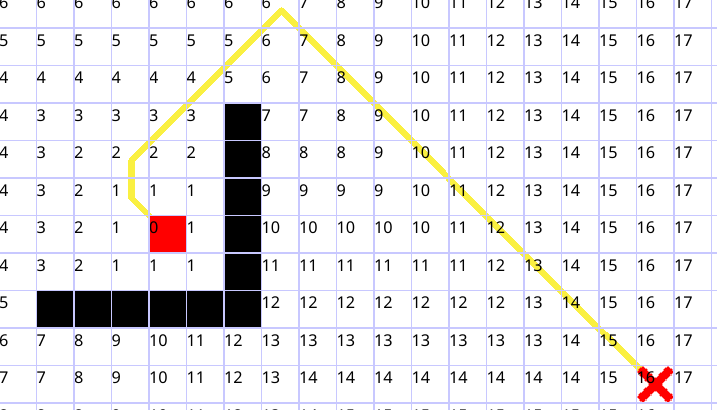
\includegraphics[width=1\linewidth]{astar-fail-dijkstra}
	\caption{Dijkstra}
\end{subfigure}
\caption{Pathfinding algorithms executed with diagonal movement allowed, and in the case of $A^*$, using the Manhattan distance as heuristic}
\label{fig:counterexample:admissible}
\end{figure}

In figure \ref{fig:node-expansion} we can see a visual comparison of the number of nodes explored using algorithms \ref{alg:dijkstra}, \ref{alg:greedy} and \ref{alg:astar} in a single example. For algorithms \ref{alg:greedy} and \ref{alg:astar}, we have used the Manhattan distance as heuristic. We can see that Dijkstra explores many more nodes than the other two (it explores even more nodes that didn't fit in the image), while Greedy Best-First Search explores many fewer nodes but the path it finds isn't optimal, since the distance of the path it calculates is $35$, while Dijkstra and $A^*$ find paths of distance $33$.

\begin{figure}
\centering
\begin{subfigure}[b]{0.45\textwidth}
	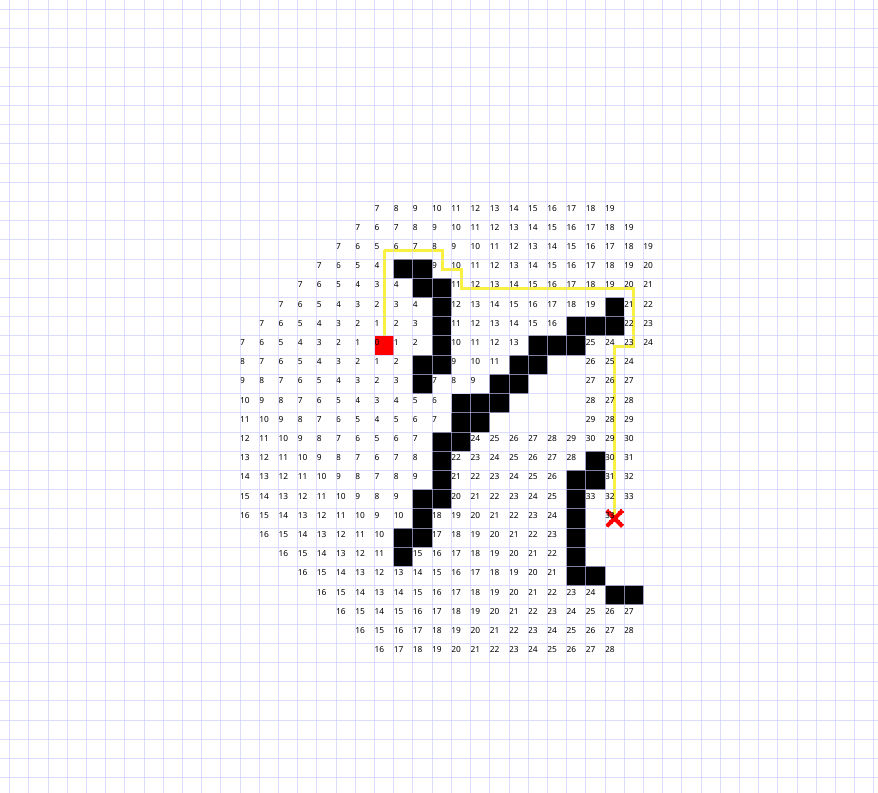
\includegraphics[width=1\linewidth]{astar-nodes}
	\caption{$A^*$}
\end{subfigure}
\begin{subfigure}[b]{0.45\textwidth}
	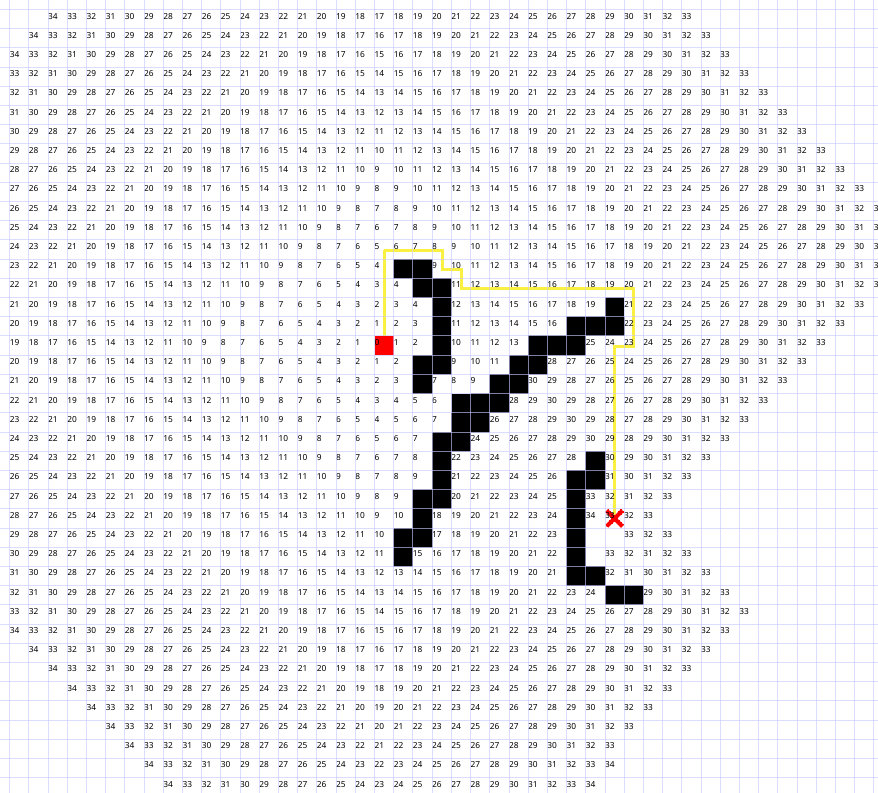
\includegraphics[width=1\linewidth]{dijkstra-nodes}
	\caption{Dijkstra}
\end{subfigure}
\begin{subfigure}[b]{0.45\textwidth}
	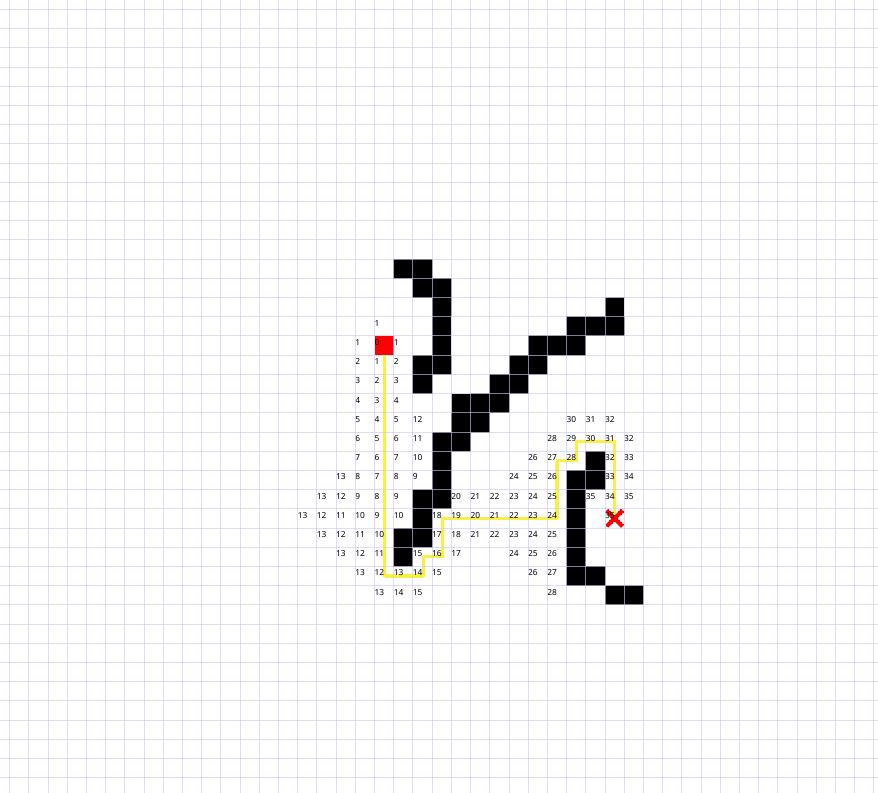
\includegraphics[width=1\linewidth]{greedy-nodes}
	\caption{Greedy Best-First Search}
\end{subfigure}
\caption{Pathfinding algorithms executed with diagonal movement allowed, and in the case of $A^*$, using the Manhattan distance as heuristic}
\label{fig:node-expansion}
\end{figure}

\chapter{Heuristics}
In the previous chapter we have proved that as long as the heuristic is admissible, $A^*$ produces optimal paths. But not any admissible heuristic will give us the same performance. Take $h(u) = 0 \  \forall u \in V$ for example, which is always admissible, and the algorithm becomes equivalent to Dijkstra, as we can see in algorithm \ref{alg:dijkstra}. We see then that $A^*$ is actually a class of algorithms, and by selecting the g-score and h-score functions we select one of the algorithms from the class. We normally only change the h-score, and use the g-score defined previously, but notice how if we make $g(u) = 0 \  \forall u \in V$, then we get another subclass of algorithms depending on the h-score which are equivalent to the Greedy Best-First Search algorithm seen in section \ref{section:greedy}. Nonetheless, when talk about $A^*$, we will usually refer to one of the algorithms in the class, after selecting an heuristic.

In this chapter, we will see that there exists an admissible heuristic which also makes $A^*$ optimal, meaning that no other pathfinding algorithm which produces optimal paths will expand fewer nodes. In practice, however, finding this perfect heuristic is often hard, but if we have enough information to constrain the set of accessible nodes 

\section{Consistent heuristics}

\begin{definition}
Given two pathfinding algorithms $A$ and $B$, we say that $A$ \textbf{dominates} $B$ if and only if both algorithms find optimal paths but the set of nodes that $A$ expands is a subset of the set of nodes that $B$ expands.
\end{definition}

\begin{definition}
Given two pathfinding algorithms $A$ and $B$, we say that $A$ \textbf{strictly dominates} $B$ if and only if $A$ dominates $B$ and $B$ does not dominate $A$.
\end{definition}

\begin{definition}
Given a class of algorithms $\bar{A}$, we say that $A \in \bar{A}$ is \textbf{optimal} if and only if $A$ dominates every member of $\bar{A}$.
\end{definition}

\begin{definition}
A heuristic $h$ is said to be \textbf{consistent} or monotone if and only if, $\forall u, v \in V$ satisfy
\[ h(u) \leq \delta(u, v) + h(v) \]
which is a form of the more general triangle inequality, and it also satisfies $h(\beta) = 0$ where $\beta$ is the goal node.
\end{definition}

\begin{proposition}
\label{prop:consistent}
Given an heuristic $h$,
\[ h \text{ is consistent} \Rightarrow h \text{ is admissible} \]
\end{proposition}
\begin{proof}
Let $\beta \in V$ be the goal node of the heuristic $h$. We will prove that $\forall u \in C_\beta$, $h(u) \leq \hat{h}(u)$, by induction on the number of steps from $u$ to the goal in an optimal path $P$.

Let $u \in C_\beta$, and let $P$ be an optimal path from $u$ to $\beta$. If there are 0 steps from $u$ to $\beta$ in $P$, then $u = \beta$, and $h(u) = h(\beta) = 0 \leq \hat{h}(u) = 0$.

Now suppose that $u$ is $k > 0$ steps away from $\beta$ in $P$. Let $v$ be the successor of $u$ in $P$, which is $k-1$ steps away from $\beta$. Therefore, since $h$ is consistent,
\[ h(u) \leq \delta(u, v) + h(v) \]
But by our inductive hypothesis, $h(v) \leq \hat{h}(v)$, and therefore
\[ h(u) \leq \delta(u, v) + \hat{h}(v) = \hat{h}(u) \]
since $P$ is an optimal path.
\end{proof}

The converse is not true in general, although in practice it can be difficult to find an admissible heuristic that is not also consistent. We will show this with a counterexample. Take the graph from figure \ref{fig:heuristic}, and let $C$ be the goal node. Let's define the heuristic as
\begin{align*}
h(A) &= 4\\
h(B) &= 1\\
h(C) &= 0
\end{align*}
The heuristic is clearly admissible, since $h(A) \leq \hat{h}(A) = 4$, $h(B) \leq \hat{h}(B) = 3$, and $h(C) \leq \hat{h}(C) = 0$. But it is not consistent, since $h(A) > \delta(A, B) + h(B) = 1 + 1 = 2$.

\begin{figure}
\centering
\begin{tikzpicture}
	[scale=.8, auto, node_style/.style={circle, draw=blue, fill=blue!20},
	edge_style/.style={draw=black, ultra thick}]
	\node[node_style] (n1) at (-5,0) {A};
  	\node[node_style] (n2) at (0,0) {B};
  	\node[node_style] (n3) at (5,0) {C};
  	
  	\draw[edge_style] (n1) edge node{1} (n2);
  	\draw[edge_style] (n2) edge node{3} (n3);
\end{tikzpicture}
\caption{A weighted undirected graph.}
\label{fig:heuristic}
\end{figure}

We will prove that with a consistent heuristic, $A^*$ is optimal. By proposition \ref{prop:consistent} we see that consistency is a stronger condition than admissibility, and therefore by theorem \ref{thm:astar}, the algorithm will still find optimal paths.

%TODO make proof of optimality

\chapter{$A^*$ variants}

\section{$IDA^*$}
Iterative Deepening $A^*$, or $\bm{IDA^*}$, is a variant of $A^*$ based on iterative deepening search, which is a modification of Depth-First Search that finds the best depth limit. %TODO talk about DFS in the annex


%TODO make chapter on tie-breaking rules

\end{document}
